\chapter{Delay}
\graphicspath{{foto/Chap2/}}

\section{Delay computation}
\subsection{Precharge \& Read operation}
In the following we compute the delay due to a precharge operation followed by a read operation involving just one read port.

\subsubsection{Precharge unit delay}
\label{sec:precharge_unit_delay}
The precharge unit is driven by an \textit{Enable} signal coming from a control unit internal to the memory (which we won't consider in this analysis). It is built by a pmos transistor for each bitline, connected from one side to the supply voltage and from the other side to the bitline, plus an equalizer pmos transistor between the two bitlines. The aim of the equalizer is to avoid that small differences in the equivalent resistance of each precharge pmos may induce some differences in the delay of the precharge operation, or equivalently in the value of the voltage reached by the two precharged bitlines. 

The scheme of the unit is the following:

\begin{center}
	\begin{figure}[H]
		\centering
		\includegraphics[scale = 0.8]{prechargeunit.png}
		\caption{Scheme of the precharge unit}
	\end{figure}
\end{center}

The \textit{Enable} signal, called \textit{PRE\#} in the figure, has to discharge the gate capacitance of these three pmos, in order to make them able to switch, so the delay associated to this operation is:
$$\tau=R_{ext,pu,driver}(C_{ext,pu,driver}+2\cdot C_{g,pre}+C_{g,equalizer})$$\\

After the switching of the precharge unit, the bitline takes a certain time to be charged. This delay is computed using the Bakoglu model: 
$$\tau=[R_d(C_d+C_w+C_L)+R_wC_L]+\frac{0.377}{0.69}(R_wC_w)$$
$R_d=R_{eq,pre,p}$ is the equivalent resistance of the driver, here equal to the resistance of the driving pmos transistor; $C_d=C_{s,pre}$ is the self-load capacitance of the driver, equal to the source capacitance of the same pmos transistor. $R_w=r\cdot l$ and $C_w=c\cdot l$ are the resistance and capacitance of the bitline, computed respectively from the resistance and capacitance per unit of length, where $l=BL_{length}$: here $r=BL_{r}$, resistance per unit of length of the bitline, and $c=BL_{c}+C_{d,access,l}$, where the first term is the capacitance per unit of length of the bitline, and the second term is the capacitance per unit of length due to the access transistor connecting each memory cell to the bitline. Finally, the load capacitance $C_L=(C_{d,sa,p}+C_{d,sa,n}+C_{g,sa,p}+C_{g,sa,n})+C_{d,blockpass}$ takes into account, with the first four terms, the capacitance due to the presence of the sense amplifier connected to each couple of bitline, and with the second term the self-load capacitance of the pass transistor at the end of each bitline.

\subsubsection{Block decoder delay}
To model the delay of this and of the other similar components we used the classical model used to determine the delay of a logic gate. The dynamic NAND decoder, in fact, is built by a precharge pmos followed by a stack of nmos transistors, as in the following picture:

\begin{center}
	\begin{figure}[H]
		\centering
		\includegraphics[scale = 0.6]{NANDdec.png}
		\caption{Core of the dynamic NAND decoder}
	\end{figure}
\end{center}

Only one among these stacks of transistors will switch, making the corresponding output to go low, and so the whole structure behaves just like an ordinary logic gate.

In addition to this structure, of course, we have also the inverters placed on the input, to get also the complemented version of the address bits. Moreover, we also have a set of inverters on the output lines: the active output of a NAND decoder, in fact, is low; the output lines of the block decoder instead, as can be observed from the full scheme of the memory reported below for convenience, are needed to switch one of the nmos transistors which connect the output from the row decoder to the wordlines, and of course the nmos transistors are turned on by a high voltage. 

\begin{center}
	\begin{figure}[H]
		\centering
		\includegraphics[scale=0.15]{REG_FILE-BLOCK_SCHEME.png}
		\caption{Full scheme of the memory}
		\label{block_scheme}
	\end{figure}
\end{center}

We consider the address bits in input to the block decoder, including their complemented version, to be stable from the beginning, while we have to take into account the delay contribution due to the inverters on the output lines. 

As mentioned before, we model this delay contribution like the delay of a traditional logic gate, so:
$$\tau_{block,dec}=R_n(C_d+C_L)$$
$R_n=Stack_n\cdot R_{eq,bdec,n}$ is the equivalent output resistance due to the stack of the nmos transistors, where $R_{eq,bdec,n}$ is the output resistance of a single nmos transistor and $Stack_n=Block\_Address$ is the number of nmos transistors forming the stack. $C_d=C_{d,bdec,pcharge}+C_{d,bdec,eval}$ is the self-load capacitance due to the drain-bulk capacitance of the pmos and of the nmos on the output line. $C_L=C_{g,bdec,inv,p}+C_{g,bdec,inv,n}$ finally is the load capacitance due to the presence of the inverter on the output line. 

\paragraph{Output inverter delay}
The delay of the inverter on the output line is computed following the same model: 
$$\tau_{block,inv}=R_p(C_d+C_L)$$
$R_p=1\cdot R_{eq,bdec,inv,p}$ is the output resistance of the inverter; here we have focused on the pmos because we are interested in the case in which its output is driven high, since that is the only case where it is able to switch the gate capacitance of the pass transistor it has as a load. $C_d=C_{d,bdec,inv,p}+C_{d,bdec,inv,n}$ as usual is the self-load capacitance of the gate. $C_L=N_{wl}C_{g,rowpass}+2N_{bit}C_{g,blockpass}$ is the full load of each inverter on the output of the block decoder. This inverter in fact has to drive the $N_{wl}$ pass transistors connected to the wordlines (row pass transistors), plus the pass transistor which allows the word just read to go out from the block (block pass transistors; hence the $+2N_{bit}C_{g,blockpass}$). Notice in fact that in the scheme we're analysing there is no column decoder; this component would be necessary if along a single row of each block of the memory there were more than one word; since we're assuming instead that each row hosts only a single word, the column decoder is useless and can be avoided. 

\subsubsection{Row decoder delay}
The next contribution is the one due to the row decoder. The block decoder and the row decoder work together, but if the number of address bits in input to the row decoder is much larger than the ones in input to the block decoder (and this is likely), also the stack of the nmos transistor will be larger and the row decoder will result to be slower than the block decoder. However, the block decoder has a load capacitance considerably higher than the one of the row decoder: not only it drives more transistors, but the capacitance to be considered in its case is the gate capacitance, which is much larger than the drain capacitance of the same transistor. So, since we don't know, at least using parametric values, which delay will be larger, we decided to compute both and to consider at the end, in the final value of the delay, only the largest between the two. The difference, as said, may be either in the contribution due to the decoder structure or in the contribution due to the driving capabilities of the inverter on the output line: for example, the block decoder may have a lower number of stack transistor, but the load of its inverter may be much larger. So, in the end, we must compare separately $\tau_{block,dec}$ with $\tau_{row,dec}$ and $\tau_{block,inv}$ with $\tau_{row,inv}$. The critical path delay will be determined by the largest from each couple of comparisons. We sum up below the structural details interested in this analysis for sake of clarity.

\begin{center}
	\begin{figure}[H]
		\centering
		\includegraphics[scale=0.6]{blockrowdec.png}
		\caption{Row decoder and block decoder timing}
	\end{figure}
\end{center}

Since the structure of the decoder is the same, also the model to compute its delay doesn't change:
$$\tau_{row,dec}=R_n(C_d+C_L)$$
$R_n=Stack_n\cdot R_{eq,rdec,n}$ is the equivalent resistance due to the stack of the nmos transistors, and $Stack_n=Row\_Address$. $C_d=C_{d,rdec,pcharge}+C_{d,rdec,eval}$ is the self-load capacitance. $C_L=C_{g,rdec,inv,p}+C_{g,rdec,inv,n}$ is again the load capacitance due to the inverter on the output.

\paragraph{Word line delay}
The inverter on the output of the row decoder is taken into account in this section, since it works as driver for the charge of the selected word line. Due to the presence of the pass transistor between the row decoder and the word line, which represents the load to be charged, we have to use the Elmore model to represent the situation.

\begin{center}
	\begin{figure}[H]
		\centering
		\includegraphics[scale=0.6]{wordlinedelay.png}
		\caption{Elmore model for the wordline delay}
	\end{figure}
\end{center}

Each memory cell is connected to the wordline through the gate of the two access transistors. So, the load $C_L$ to be charged can be computed as $C_L=2C_{g,access,l}\cdot WL_{length}$, where $C_{g,access,l}$ is the gate capacitance of a single access transistor per unit of length and $WL_{length}$ is the length of the wordline.

The equation to compute the delay with the Elmore model becomes:
$$\tau_{row,inv}=R_{eq,inv}(C_{d,inv}+C_{d,pass}+C_L)+R_{eq,pass}(C_{d,pass}+C_L)$$
$R_{eq,inv}=R_{eq,rdec,inv,p}$ is the equivalent resistance from the output of the inverter (again, we focus on the pmos because the interesting case is when its output goes high). $C_{d,inv}=C_{d,rdec,inv,p}+C_{d,rdec,inv,n}$ is the self-load capacitance of the inverter. $R_{eq,pass}=R_{eq,rowpass}$ and $C_{d,pass}=C_{d,rowpass}$ are respectively the equivalent resistance and drain capacitance of the pass transistor which drives the wordline. $C_L=2C_{g,access,l}\cdot WL_{length}$ is the total load capacitance for each wordline, as described above. \\

Before analysing the delay due to the reading of the value stored inside the cell, we insert a brief review about the functioning of the SRAM memory cell, and the constrains we have on the transistors size. 

\subsubsection{SRAM memory cell}
\label{subsec:SRAM_memory_cell}
The structure of the cell, assuming to have two read ports and one write port, is the following:

\begin{center}
	\begin{figure}[H]
		\centering
		\includegraphics[scale = 0.4]{sramcell.png}
		\caption{Structure of a SRAM cell}
	\end{figure}
\end{center}

Let's say we want to read with the \textit{port1} a value 0 stored in the cell: then M1 and M4 are turned on, while M2 and M4 are off. After precharging both bitlines to \textit{Vdd} and activating $WL_{read1}$, \textit{BL1} will be discharged through the series of M1 and M5 (remember that, to avoid errors, we must have that $W_1>W_5>W_2$). So, the huge bitline capacitance (capacitance per unit of length including $BL_c$ and the capacitance per unit of length due to the access transistors, plus the input capacitance of the sense amplifier and the drain capacitance of the column pass transistor) will be discharged through the series of those two transistors. However, thanks to the sense amplifier, we don't need to wait the full discharge, because after only few percents of the full \textit{Vdd} voltage swing the sense amplifier will go out its metastable state and will accelerate the transition. We indicate these "few percents" with the parameter $K_{SA}$. 

If instead we are trying to write, let's say, a 1 into the memory cell, while for example the stored value is 0 (so, M1 and M4 on, M2 and M3 off): first of all we must force the value 1 and 0 respectively on $BLW$ and $BLW^*$ with an external driver. M9 and M10 will be turned on by $WL_{write}$: since M4 is more resistive than M10, the node between M4 and M10 will be discharged through the resistance of M10; as soon as the voltage on that node goes below the threshold of the inverter composed by M1 and M2, M2 will turn on while M1 turns off, so that also the node connected to M9 switches from 0 to 1 and also the value previously imposed on \textit{BLW} is correctly stored inside the cell. 

\paragraph{Bit line delay} 
\label{sec:bitline_delay}
So, during the read operation, the memory cell acts as a driver on a huge capacitance. However, as said, we can consider only a portion $K_{SA}$ of the whole delay thanks to the sense amplifier. 

We can compute the delay due to the read operation applying the Bakoglu model:
$$\tau=[R_d(C_d+C_w+C_L)+R_wC_L]+\frac{0.377}{0.69}(R_wC_w)$$
$R_d=R_{eq,cell,n}+R_{eq,access,n}$ is the equivalent resistance of the driver, which this time is the memory cell; $C_d=C_{d,access}$ is the capacitance associated to the driver, equal to the drain capacitance of the access transistor. $R_w=r\cdot l=BL_{r}\cdot BL_{length}$ is the total resistance of the bitline, while $C_w=c\cdot l=(BL_{c}+C_{d,access,l})BL_{length}$, like in the case of the precharge. Finally, the load capacitance is again $C_L=(C_{d,sa,p}+C_{d,sa,n}+C_{g,sa,p}+C_{g,sa,n})+C_{d,blockpass}$.

Including also the $K_{SA}$ factor, the equation becomes: 
$$\tau=K_{SA}\{[R_d(C_d+C_w+C_L)+R_wC_L]+\frac{0.377}{0.69}(R_wC_w)\}$$

\subsubsection{Sense amplifier delay}
The sense amplifier is made with two cross coupled inverters that are brought to a metastable state and then are applied a voltage difference by means of the input bitlines. Notice that in this amplifier input and output are somehow coincident. The schematic of the component is shown below:

\begin{figure}[h] 
	\begin{center}
		\includegraphics[scale=0.4]{senseamplifier.png}
	\end{center}
	\caption{Sense amplifier structure} 
\end{figure}

Its delay is described by a simple RC model:
$$\tau=R_{eq,sa,mod,parallel}[C_{d,sa,p}+C_{d,sa,n}+C_{g,sa,p}+C_{g,sa,n}+(BL_c\cdot BL_{length})+C_{d,blockpass}]$$
In this equation we take into account the equivalent resistance of the sense amplifier, which drives its self-load capacitance, the capacitance due to the gate of the cross-coupled inverter, the capacitance of the bitline, plus the drain capacitance of the pass transistor connected at the bottom of the bitlines and whose gate terminal is driven by the block decoder.

\subsubsection{Delay of the column pass transistor}
Finally, the last contribution to the delay is given by the pass transistor (one for each bitline) we have before the output from the block. It is driven by the block decoder (by the inverter on its output). To estimate the delay associated to this component is enough to compute:
$$\tau=R_{eq,pass}(C_{d,pass}+C_L)$$
$R_{eq,pass}=R_{eq,colpass}$ is the equivalent resistance of the pass transistor, whereas $C_{d,pass}=C_{d,blockpass}$ is its self-load capacitance. $C_L$ is unknown and in our analysis is assumed to be an open circuit. 

\subsubsection{Total delay}
The total delay is computed as the sum of all the contributions described up to now (with the exception of the block decoder and the row decoder, as already described), multiplied by 0.69.

\subsection{Write operation}
Having already analysed all the contributions to the delay associated to a read operation, analysing the delay of a write operation is very simple. First of all, we give as input to the block and to the row decoder, both specific for the write operation, the address of the row where we want to write the word provided on input of the memory. The row decoder will activate only one of the pass transistors on its output lines, so that one of the $N_{wl}$ wordlines dedicated to the write operation will be activated. At the same time, an external driver must load the $N_{bit}$ bit to be written on the bitlines. Finally, as soon as the concerned $WL_{write}$ switches, the access transistors connected to it will turn on, allowing the writing of the bits into the cells along the selected row. 

So, the only differences are: the delay associated to the need to put on the bitlines the value to be stored (which however is a contribution very similar to the precharge operation; in particular, we don't consider the precharge contribution to the writing delay. The precharge before the write operation is done just to simply the control of the memory, unlike the case of a read operation, where the precharge is needed for real. So here the driver delay conceptually substitutes the precharge delay), and the delay associated to the writing of the bit inside the memory cell, operation already detailed in section \ref{subsec:SRAM_memory_cell}. A little additional difference comes from the contribution $\tau_{block,inv}$: this time in fact the load capacitance is only $C_L=N_{wl}C_{g,rowpass}$, we don't have the $+2N_{bit}C_{g,blockpass}$ term anymore. 

\subsubsection{Driver delay}
\label{sec:driver_delay}
We assume that the value of the data to be stored is forced on the bitlines before the address bits are provided in input to the decoders. In this way, the contribution due to this operation conceptually replaces the precharge operation. In principle the two operations could even happen at the same time: the driver forces the correct values on the bitlines while the decoders are still interpreting the address bits and driving their output lines consequently; however, in this second case, for data intergity reasons, we would need that $\tau_{row,dec}+\tau_{row,inv}>\tau_{driver}$ and so a very firm control on the process, because otherwise we may write a wrong value into the row: so, it is quite a dangerous assumption to do. 

We can again model this contribution with Bakoglu, just like we have done in \ref{sec:precharge_unit_delay}.
$$\tau=[R_d(C_d+C_w)]+\frac{0.377}{0.69}(R_wC_w)$$
$R_d=R_{eq,driver}$ and $C_d=C_{driver}$ are the equivalent resistance and capacitance of the external driver. $R_w=r\cdot l=BL_{r}\cdot l$ and $C_w=c\cdot l=(BL_{c}+C_{d,access,l})\cdot l$ are the resistance and capacitance of the bitline. Here we don't have any "lumped" load capacitance $C_L$. 

\subsubsection{Cell delay}
As already described in section \ref{subsec:SRAM_memory_cell}, we assume to be writing a 1 into a memory cell currently containing a 0. Due to the constrains on the width of the transistors internal to the cell ($W_1>W_9>W_2$ and $W_3>W_{10}>W_4$), we only able to write a 0, not a 1, so we have to consider first the right side of the cell, related to $BLW^*$. The transistor $M_4$ is on, the bitline $BLW^*$ is hosting the value 0, and $M_{10}$ is trying to discharge the node it has in common with $M_4$. The situation then can be summed up like:

\begin{minipage}{\linewidth}
\centering
	\begin{minipage}{0.3\linewidth}
		\begin{figure}[H]
			\begin{center}
				\includegraphics[scale=0.3]{writecell.png}
			\end{center}
				\caption{Equivalent circuit for the first half of the write delay} 
		\end{figure}
	\end{minipage}
	\hspace{0.05\linewidth}
	\begin{minipage}{0.6\linewidth}
		\begin{figure}[H]
			\begin{center}
				\includegraphics[scale=0.3]{sramcell.png}
			\end{center}
				\caption{SRAM cell}
		\end{figure}
	\end{minipage}
\end{minipage}\\

$R_1$ and $R_2$ are related respectively to $M_4$ and $M_{10}$ (we report the same picture of the memory cell already shown for convenience), and $R_1>R_2$. $C$ is the capacitance of the node between the two transistors and is equal to $C_{g,cell,p}+C_{g,cell,n}+C_{d,cell,p}+C_{d,cell,n}+C_{s,access}$. The time constant of this circuit is equal to $$\tau_1=\frac{R_1R_2}{R_1+R_2}\cdot C$$
This means that the capacitor $C$ will be charged with this time constant. As soon as the voltage on the node goes above the threshold of the inverter composed by $M_1$ and $M_2$, the inverter will take a certain time to switch, while charging the capacitance related to the node in common between the access transistor $M_9$, $M_1$ and $M_2$. Only at this point the value is correctly stored inside the cell and the operation ends. This "certain time" can be computed like: $$\tau_2=R_{eq,cell,p}\cdot C$$
$R_{eq,cell,p}$ is the resistance of the pmos transistor $M_2$, while $C$ is symmetrical to the capacitance represented in the picture above and has the same expression. 

Since we don't know the value for the threshold of the inverter, we assume that this value is reached after $4\tau_1$. Then, the total delay associated to the writing of the value inside the memory cell is equal to
$$\tau=4\tau_1+\tau_2$$

\section{Simulation results}
To verify the plausibility of our computations we assigned a reasonable value to each of the parameters involved in the equations. We also made the number of bits, contained in each word hosted in the memory change, in a well defined range, in order to analyse how the delay changes if we vary the dimensions of the memory array. In particular, we considered $N_{word}=128$ and $N_{bit}$ in the range $[8, 16, 32, 64, 128]$.\\

The results we obtained are reported in the figures below. In particular, in fig. \ref{delay_read} is shown the delay we have with a read operation. We can notice a more than linear behaviour with the increase of $N_{bit}$. The reason for this is in the usage of the Bakoglu model in sections \ref{sec:precharge_unit_delay} and \ref{sec:bitline_delay}. In particular, the distributed term inside the Bakoglu equation involves a $BL_{length}^2$ contribution, and we must remember that $BL_{length}$ depends linearly on the variable $N_{bit}$. To verify our reasoning we commented the lines of code involving the Bakoglu delay computation and we found a linear behaviour, as we expected. 

We can also notice that, with the choice of values we have made, the expected value for the read delay spans between $0.16ps$ for $N_{bit}=8$ and $12.4ps$ for $N_{bit}=128$. 

\begin{figure}[H]
	\begin{center}
		\includegraphics[scale=0.4]{delay_read.eps}
	\end{center}
	\caption{Delay on a read operation} 
	\label{delay_read}
\end{figure}

In fig. \ref{delay_write} we report the simulation concerning the delay on the write operation. As already said, in the delay computation of a write operation, the precharge is substituted by the writing of the values to be stored on the bitlines; the block and the row decoder contributions remain the same, with the only difference that here the load of the inverter on the output of the block decoder is a bit lower; finally, we have a different delay associated to the writing of the value inside the memory cell, while we don't have the contributions of the sense amplifier and of the pass transistor at the end of the bitlines. So, overall, we expect to have a result a bit lower with respect to the delay associated to the read operation.
 
\begin{figure}[H]
	\begin{center}
		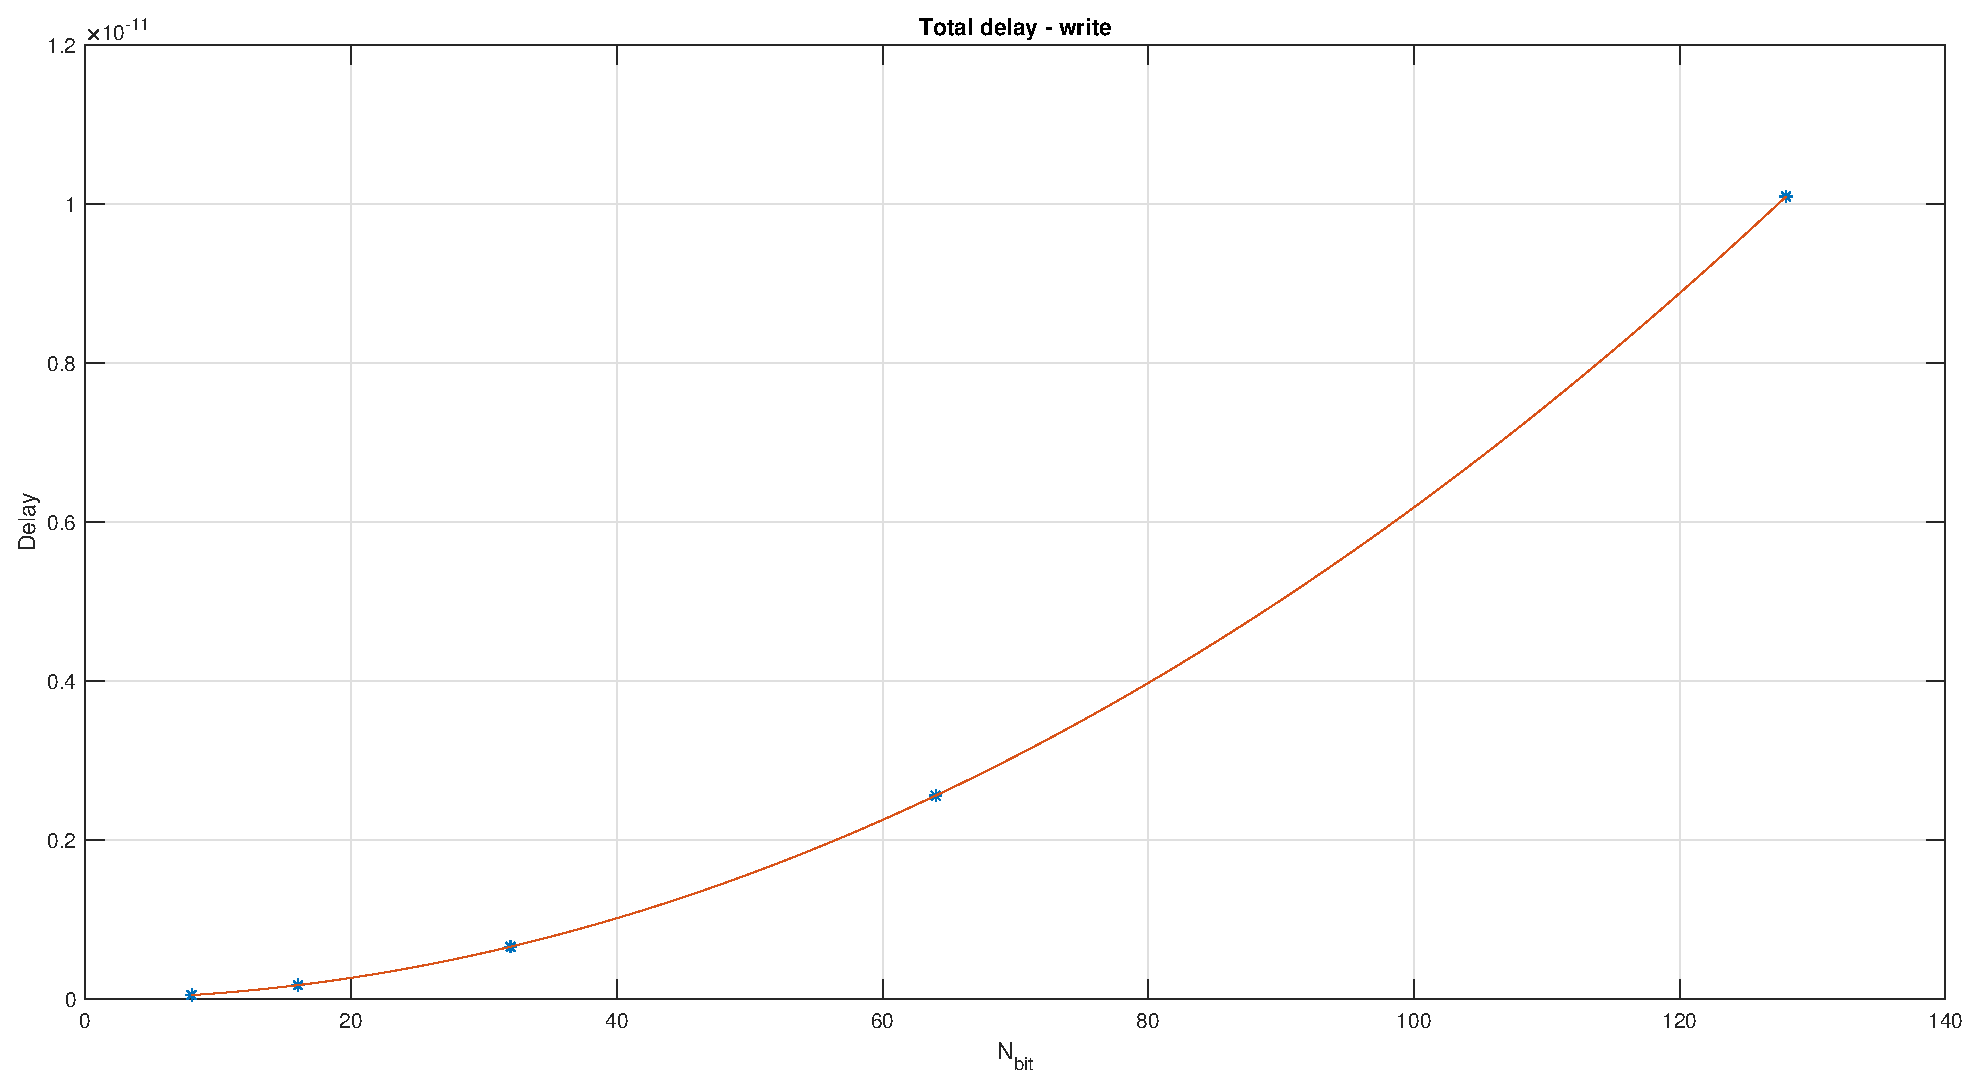
\includegraphics[scale=0.4]{delay_write.eps}
	\end{center}
	\caption{Delay on a write operation}
	\label{delay_write}
\end{figure}
	
We can observe again a more than linear behaviour, due to the use of the Bakoglu model in sec. \ref{sec:driver_delay}. For $N_{bit}=8$ we have a delay of $0.047ps$ (after all, in this case we have a register file divided in 16 blocks of 8 words with 8 bits each, so each memory array is very small), while for $N_{bit}=128$ we have a delay of about $10ps$.